% !TeX root = ../economia.tex
\chapter{Valutazione degli Investimenti}

\section{Introduzione}
Il \emph{flusso di capitale} in un'azienda si articola nelle seguenti fasi:
\begin{enumerate}
    \item Gli \emph{azionisti} versano capitale nell'\emph{impresa}
    \item L'\emph{impresa} investe il capitale per realizzare \emph{progetti di investimento}
    \item L'attività dell'impresa genera \emph{cassa}
    \item Parte della \emph{cassa} viene usata per autofinanziare nuovi progetti
    \item Parte della cassa viene distribuita agli azionisti come \emph{dividendi}
\end{enumerate}

Per finanziarsi, un'azienda si avvale di \emph{istituti di credito}, che erogano
\emph{finanziamenti}, debiti (\emph{oneri finanziari}) che verranno ripagati dall'azienda.

\section{Politiche di investimento}
Un'\gls{investimento} è  tipicamente una decisione rilevante per l’impresa, che
ha effetti economici significativi (tali da giustificarne il \emph{rischio}) e
\emph{dilazionati} nel tempo, quindi incerti.

In particolare:
\begin{itemize}
    \item \textbf{È difficilmente reversibile:} un investimento richiede, solitamente, notevoli impieghi iniziali di denaro
    \item \textbf{Ha un impatto temporale di lungo periodo:} gli esiti dell’investimento si hanno lungo un orizzonte temporale ampio
    \item \textbf{Ha un effetto economico incerto:} genera risultati dagli esiti incerti
\end{itemize}

\subsection{Concetti preliminari (con esempi)}
\begin{itemize}
    \item \textbf{\Gls{rendinvest}}: L’investitore compra un’azione di una certa impresa pagando $100$.
    A fine anno guarda il valore di tale azione sul mercato, scoprendo che è salito a $110$.
    In più, durante l’anno ha ricevuto dividendi per un valore di $5$.
    Il valore finale dell’investimento è $110 + 5 = 115$.

    $\rightarrow$ Rendimento $ = 15\%$

    \item \textbf{\Gls{riscinvest}}: Invece di avere un prezzo finale di $110$, l’azione vale solo $80$.
    Tenendo conto dei dividendi pari a $5$, il valore finale dell’investimento è $80 + 5 = 85$.

    $\rightarrow$ Rendimento (negativo) $= -15\%$
\end{itemize}

\textbox{
I rendimenti futuri (incerti) associati all’investimento valgono i costi iniziali
(certi e/o onerosi)?
}

\subsection{Esempi di decisioni di investimento \emph{finanziarie}}
\begin{itemize}
    \item \textbf{Investimenti in attività finanziarie:}
    Il prezzo del titolo (azione, obbligazione) è adeguato?
    \item \textbf{Investimenti in attività reali:}
    Il valore dell’immobile che sto acquistando è commisurato al prezzo di vendita?
    \item \textbf{Finanziamento bancario:}
    Il costo di finanziamento è commisurato alla redditività che lo stesso riesce a generare?
    \item \textbf{Destinazione degli utili d’impresa:}
    E’ meglio distribuire dividendi o re-investire le risorse nell’azienda?
\end{itemize}

\subsection{Esempi di decisioni di investimento \emph{tecniche}}
\begin{itemize}
    \item \textbf{Espansione:}
    Acquistiamo un nuovo impianto o un nuovo stabilimento in aggiunta a quelli già disponibili?
    \item \textbf{Sostituzione:}
    Conviene sostituire gli impianti esistenti?
    \item \textbf{Scelta di tecnologia:}
    Quale dei diversi possibili macchinari/impianti scegliamo per un certo scopo?
    \item \textbf{Ampliamento dell’offerta (sviluppo di nuovi prodotti):}
    Aggiungiamo un prodotto all’attuale gamma?
    Entriamo o meno in un nuovo mercato?
\end{itemize}

\section{Valore attuale netto (VAN)}
Il Valore Attuale Netto (\gls{VAN}) o Net Present Value (NPV) rappresenta la
\emph{somma dei flussi di cassa netti}, cioè i benefici ($=$ ricavo $-$ costi), che un investimento
è in grado di generare tenendo in considerazione il fattore \emph{tempo} e \emph{rischio}.

Il \gls{VAN} dipende quindi da:
\begin{itemize}
    \item L’ammontare dei net cash flows (\gls{NCF}) stimati generati dall’investimento
    \item Gli istanti di tempo nei quali i \gls{NCF} vengono generati
    \item L’incertezza (rischio) associata ai \gls{NCF}
\end{itemize}

Poiché l’investimento ha impatti di lungo periodo, i flussi finanziari sono
localizzati in \emph{istanti temporali differenti} quindi \emph{non sono direttamente sommabili}.

Attraverso il meccanismo di \emph{attualizzazione} rendiamo comparabili flussi di denaro
localizzati in istanti di tempo differenti e con diversi livelli di rischio.

\subsection{Fattore tempo}
Consideriamo un ``mondo'' in cui esistano solo investimenti ``certi'' (privi di rischio)
e chiamiamo $i$ il tasso di rendimento di questi investimenti.
Se disponiamo adesso di una somma $X(0)$, possiamo investirla a un tasso pari a $i$.

Dopo un periodo di tempo $t$, disporremo con certezza di una cifra superiore, pari a
\[X(t) = X(0) + X(0) \times i\]

È quindi indifferente disporre al periodo $t=0$ di $X(0)$ oppure al periodo $t=1$ di una cifra
\[X(1) = X(0)\times(1+i)\]

Se manteniamo il nostro denaro nell’investimento per un altro periodo, disporremo al periodo $t=2$ di
\[X(2) = X(1)*(1+i) = X(0)*(1+i)^2\]

Iterando il procedimento, otteniamo che il valore futuro, in un periodo $t$ generico, di una somma $X(0)$
disponibile attualmente è dato dalla formula di capitalizzazione, mentre la sua inversa,
la formula di attualizzazione, ci permette di calcolare il valore attuale $X(0)$ di una somma di denaro $X(t)$ disponibile
tra $t$ anni.
\begin{multicols}{2}
    \paragraph{Formula di capitalizzazione}
    \[X(t) = X(0)*(1+i)^t\]
    
    \paragraph{Formula di attualizzazione}
    \[X(0) = \frac{X(t)}{(1+i)^t}\]
\end{multicols}

\subsection{Fattore tempo + rischio}

Assumiamo di essere \emph{avversi al rischio}, ovvero che preferiamo disporre di \emph{somme certe} piuttosto che incerte
e che accetteremo investimenti rischiosi solo se ci aspettiamo un \emph{rendimento superiore} di quello degli
investimenti privi di rischio. Introduciamo $d$, che rappresenta il \emph{premio per il rischio}, ovvero l’incremento nel rendimento richiesto per compensare il
rischio associato al futuro.
\begin{multicols}{2}
    \paragraph{Formula di capitalizzazione}
    \[X(t) = X(0)\times(1+i+d)^t\]
    
    \paragraph{Formula di attualizzazione}
    \[X(0) = \frac{X(t)}{(1+i+d)^t}\]
\end{multicols}

\subsection{Tasso di sconto (rendimento)}
Se definiamo $k=i+d$ come \emph{tasso di sconto}, possiamo definire il \emph{fattore di sconto}
\[\text{Fattore di sconto} = \frac{1}{(1+k)^t}\]

Il fattore di sconto corrisponde al valore attuale ($t=0$) di \euro 1 ottenuto al tempo $t$.

Se moltiplico il fattore di sconto per il flusso di cassa, ottengo il valore attuale di quel flusso di cassa.

$I_0$ indica l'investimento iniziale.
\begin{equation*}
    \text{\gls{NCF}}(t) = \text{Entrate di cassa}(t) - \text{Uscite di cassa}(t)
\end{equation*}
\begin{equation*}
    \text{VA (Valore Attuale)} = \text{fattore di sconto} \times \text{NCF} = \frac{\text{NCF}}{(1+k)^t}
\end{equation*}
\begin{equation*}
    \text{\gls{VAN}} = -I_0 + \text{VA}
\end{equation*}

\subsection{VAN di un progetto di investimento}

Il \gls{VAN} è la somma di tutti i \gls{NCF} differenziali, in valore attuale, al \emph{netto} dell’investimento iniziale $I_0$.

\begin{equation*}
    \text{VAN} = \sum^T_{t=0} \frac{\Delta\text{NCF}_t}{(1+k)^t}
    = \sum^T_{t=1} \frac{\Delta\text{NCF}_t}{(1+k)^t} - I_0
    = \text{PV} - I_0
\end{equation*}

\begin{itemize}
    \item Se VAN $> 0$, l’investimento crea valore e all’impresa conviene intraprendere il progetto di investimento.
    \item Se VAN $= 0$, per l’impresa è indifferente intraprendere o meno il progetto di investimento.
    \item Se VAN $< 0$, l’investimento distrugge valore e all’impresa non conviene intraprendere il progetto di investimento.
\end{itemize}

Talvolta uno degli aspetti critici nella valutazione del VAN è dato dalla definizione dell’orizzonte temporale di
riferimento: l’investimento infatti, essendo una decisione di lungo periodo, ha effetti significativi
sull’impresa su un arco di tempo limitato, ma può anche avere impatti successivi fino a $t = +\infty$.

In questo caso, è opportuno dividere la formula in due orizzonti temporali di riferimento:
\begin{itemize}
    \item $0 \rightarrow T$: orizzonte di previsione, orizzonte temporale per il quale è possibile esprimere previsioni “ragionevoli” e puntuali sugli impatti dell’investimento in termini di creazione di valore
    \item $T \rightarrow +\infty$ concretizzato in un’unica grandezza che esprime il valore dei NCF successivi all’anno $T$, che
    chiamiamo \emph{valore residuo} o \emph{valore terminale}:
    \begin{equation*}
        \text{Valore residuo} = \frac{V(t)}{(1+k)^T} \quad\longrightarrow\quad
        \text{VAN} = \sum_{t=1}^T \frac{\Delta \text{NCF}_t}{(1+k)^t} + \frac{V(t)}{(1+k)^T}
    \end{equation*}
\end{itemize}
\paragraph{Investimento con rendita perpetua (serie geometrica)}
\begin{equation*}
    \text{VAN} = -I_0 + \frac{C}{k}
\end{equation*}
dove $I_0$ è l'investimento iniziale, $C$ è il flusso di cassa, $k$ è il tasso di sconto.

\paragraph{Investimento con rendita perpetua crescente a tasso costante} con tasso $g < k$
\begin{equation*}
    \text{VAN} = -I_0 + \frac{C}{k-g}
\end{equation*}

\paragraph{Investimento con rendita annuale costante} es.: mutuo
\begin{equation*}
    \text{VAN} = -I_0 + \frac{C}{k} \left(1-\frac{1}{(1+k)^T}\right)
\end{equation*}

\section{Stima dei NCF}
Il primo passo nella valutazione di un investimento consiste nella stima dei \gls{NCF} che
esso sarà in grado di generare. La procedura si articola nelle seguenti fasi:

\subsection{Valutare gli effetti dell’investimento}
ll primo step nella stima dei NCF consiste nel valutare in che modo 
l’investimento influenzerebbe l’attività dell’impresa nel futuro:
\begin{itemize}
    \item Il numero, la tipologia e il prezzo dei prodotti/servizi venduti (es.: 
    cambiamenti attesi nella quota di mercato, nel mix di produzione, nel 
    margine di profitto..)
    \item Gli investimenti in immobilizzazioni (es.: macchinari e impianti) e attività 
    correnti (es. rimanenze) richiesti
    \item Marchio e reputazione dell’impresa (es.: qualità del prodotto, time to 
    market…)
    \item Qualità percepita e la soddisfazione del cliente (es.: incremento dei servizi 
    post-vendita…)
    \item Soddisfazione degli impiegati e produttività del lavoro (es.: miglioramento 
    delle condizioni di lavoro, riduzione del turnover, job enlargment e job 
    enrichment)
\end{itemize}

\subsection{Misura economica}
Il secondo step nella stima dei NCF consiste nel tradurre gli effetti reali in termini di impatto
economico. È importante osservare che l’effetto dell’investimento deve essere isolato dalle restanti attività
dell’impresa, e quindi deve essere valutato solo l’\emph{effetto differenziale} generato dallo specifico investimento in
analisi.

\subsubsection{Logica differenziale}
È necessario prendere in considerazione tutti e solo i flussi direttamente generati
dall’investimento.
Particolare attenzione deve essere rivolta alle previsioni di alcune tipologie di costi:
\begin{itemize}
    \item \textbf{Costi comuni}, ovvero quei costi che sarebbero sostenuti anche nel caso in cui non si attuasse il progetto (es. il
    personale già presente in azienda e che non potrebbe essere licenziato senza costi addizionali). \emph{Tali costi non
    devono essere considerati}
    \item \textbf{Effetti collaterali}, generati dall’attuazione di un progetto, sui flussi di cassa che si producono in altri comparti
    dell’impresa (ad esempio il lancio di un nuovo prodotto potrebbe ridurre le vendite di un prodotto già in produzione).
    Tali costi DEVONO essere considerati
    \item Erosioni: quando un nuovo progetto impatta negativamente i flussi di progetti già avviati
    \item Sinergie: quando un nuovo progetto fa aumentare i flussi di progetti già avviati 
    \item \textbf{Costi affondati} (sunk cost), ovvero quei costi, correlati allo specifico investimento, che vengono sostenuti prima
    della scelta di effettuare o meno l’investimento.
    I costi affondati non sono rilevanti nell’analisi in quanto l’impresa non ha modo di scegliere se sostenerli o meno: dal
    momento in cui l’azienda sostiene il costo, quel costo diventa irrilevante per qualunque decisione futura.
    \emph{Tali costi non devono essere considerati}
\end{itemize}


\subsection{Costo economico differenziale}
Il terzo step consiste nell’utilizzare i risultati della valutazione in termini economici degli effetti
dell’investimento per redigere un conto economico differenziale.
Le voci di conto economico che sono spesso influenzate da un investimento sono:
\begin{itemize}
    \item Ricavi
    \item Costo dei materiali
    \item Costo del lavoro
    \item Costo dei servizi
    \item Costo di manutenzione
    \item Costo dell’energia
    \item Imposte
\end{itemize}
Il contributo dell’investimento a queste voci di conto economico può essere positivo o negativo.

L’obiettivo è determinare il NCF generato dall’\emph{investimento} rispetto a quello
realizzato dall’impresa nelle condizioni attuali (prima di effettuare l’investimento).

\subsection{Calcolo dei NCF}
In questa fase si passa dalla \emph{logica economica} a quella \emph{monetaria/finanziaria}:
consideriamo solo le componenti che generano flussi di cassa nel periodo considerato.

\subsubsection{Bottom-up}
Un approccio è quello \emph{bottom-up}: aggiustamento dell’utile netto differenziale (bottom line del conto economico differenziale
creato precedentemente) generato dall’investimento per \emph{depurarlo dell’effetto delle componenti non-cash}.
L'NFC sarà dato da:
\begin{enumerate}
    \item Utile Netto differenziale
    \item $(+)$ Ammortamenti
    \item $(-)$ Plusvalenze/$+$ Minusvalenze
    \item $(-/+)$ Investimenti in immobilizzazioni
    \item $(-/+)$ Investimenti in attività correnti\footnote{investimenti in attività correnti misurati dalla \emph{variazione di capitale circolante netto} (CCN)
    \\CCN$=$ crediti commerciali $+$ scorte $-$ debiti commerciali}
\end{enumerate}

\paragraph{Ammortamenti} Gli ammortamenti rientrano tra i costi in conto economico in quanto il riconoscimento del costo di
un’immobilizzazione avviene durante la sua vita utile (anno per anno) piuttosto che essere totalmente
scontato nell’anno in cui tale immobilizzazione è stata acquistata. Tuttavia, secondo la logica finanziaria,
l’esborso avviene nell’anno di acquisto dell’immobilizzazione e
non vengono effettivamente sostenuti dei costi annui per la sua perdita di valore, pertanto l’ammortamento deve essere
sommato all’utile differenziale in modo da ricondurlo ad una logica finanziaria.

\paragraph{Plusvalenze/Minusvalenze} Quando un immobile viene venduto ad un prezzo diverso dal suo valore di bilancio la differenza tra
prezzo di vendita e valore contabile genera una plusvalenza (o minusvalenza) quando la differenza è
positiva (o negativa). Le plusvalenze devono essere sottratte all’utile di bilancio in quanto non rappresentano l’entrata di cassa,
ma, piuttosto, l’incasso aggiuntivo rispetto al valore contabile. Le minusvalenze devono essere sommate all’utile di bilancio in quanto non rappresentano un costo, ma,
piuttosto, il mancato incasso rispetto al valore contabile.

\paragraph{Investimenti} Per ottenere il NCF, dall’utile si dovranno infine scontare gli investimenti netti in immobilizzazioni e
attività correnti. Per investimenti netti in immobilizzazioni si intende:
\begin{itemize}
    \item Uscite di cassa relative all’acquisto di nuove immobilizzazioni
    \item Entrate di casse relative alla dismissione di immobilizzazioni
\end{itemize}
Per investimenti netti in attività correnti si intende:
\begin{itemize}
    \item Incremento dei crediti commerciali (che rappresentano una mancata entrata di cassa rispetto al
    conto economico), cioè un \emph{ricavo, ma non flusso di cassa}
    \item Incremento delle rimanenze di magazzino (che rappresentano una mancata entrata di cassa
    rispetto al conto economico), cioè un \emph{ricavo, ma non flusso cassa}
    \item Riduzione dei debiti commerciali (che rappresentano un’uscita di cassa aggiuntiva rispetto al
    conto economico), cioè un \emph{costo, ma non flusso cassa}
\end{itemize}

\subsubsection{Top-down}
L'NFC sarà dato da:
\begin{enumerate}
    \item EBIT differenziale
    \item $(-)$ Tasse differenziali pagate dall’impresa
    \item $(+)$ Ammortamenti
    \item $(-/+)$ Investimenti (disinvestimenti) in immobilizzazioni
    \item $(-/+)$ Investimenti (disinvestimenti) in attività correnti 
\end{enumerate}

\section{Tasso interno di rendimento (TIR)}

Il tasso di attualizzazione che annulla il valore del \gls{VAN} viene detto Tasso Interno di Rendimento (TIR) o
Internal Rate of Return (IRR) del progetto. In altri termini, il TIR corrisponde al tasso per cui il \gls{VA} dei flussi in ingresso eguaglia il VA dei flussi in
uscita.
\[
0 = -CF_0 + \frac{CF_1}{\left( 1 + IRR\right) } + \frac{CF_2}{\left( 1 + IRR\right)^2 } + \frac{CF_3}{\left( 1 + IRR\right)^3 } + \dots
\]
cio\`e, con $k$ rendimento richiesto:
\[
VAN(k = TIR) = 0
\]
\subsection{Uso del TIR}
Il TIR è un indicatore che esprime il rendimento annuo intrinseco di un progetto di investimento,
quindi facilmente confrontabile con il rendimento di investimenti alternativi (obbligazioni, azioni...):
\begin{itemize}
	\item Se TIR $> k$ (rendimento richiesto) è conveniente intraprendere il progetto di investimento
	\item Se TIR $= k$ (rendimento richiesto) è indifferente intraprendere il progetto di investimento
	\item Se TIR $< k$ (rendimento richiesto) non è conveniente intraprendere il progetto di investimento
\end{itemize}
È possibile esprimere il \gls{VAN} come funzione del tasso di attualizzazione $k$:
\[
\textit{VAN(k)} = \sum^T_{t=0} \frac{NCF_t}{(1+t)^t} - I(0) + \frac{V(T)}{(1+k)^t}
\]

\subsection{Limiti del TIR}
\begin{enumerate}
	\item Per alcuni investimenti non esiste alcun TIR, ad esempio il \gls{VAN} può essere positivo per ogni tasso di
	attualizzazione utilizzato
	\item Può non distinguere tra situazioni di investimento e di finanziamento
	\item \`E possibile la presenza di TIR multipli quando si verificano più cambiamenti di segno nei flussi di
cassa:
	
		\small{I flussi di cassa possono avere segno positivo o negativo (ad esempio un investimento successivo dopo alcuni
			anni). In questo caso, la funzione $VAN(x)$ non risulta monotona non decrescente, intersecando in più punti
			l’asse del tempo. In questo caso non è possibile attribuire un significato economico alle diverse intersezioni della funzione
			con l’asse delle ascisse}
\end{enumerate}

\subsection{Utilizzi del TIR}
\begin{itemize}
	\item Il TIR può essere considerato come il tasso di rendimento che permette di raggiungere il \emph{break-even
	finanziario} di un investimento: con un tasso di attualizzazione pari al TIR, il valore attuale netto di un
	progetto è pari a zero
	\item Il TIR è frequentemente utilizzato in quanto permette ai manager finanziari e agli analisti di valutare le
	performance in termini relativi, come ``12\%'', piuttosto che in termini assoluti, come ``46 000''\euro
	\item Il metodo del TIR è preferito a quello del VAN nei casi in cui il tasso di attualizzazione dei flussi è
	non noto o soggetto ad incertezza; in queste situazioni il TIR fornisce maggiori informazioni su un
	investimento di quanto possa fare il VAN
	\item Nei casi in cui il tasso di attualizzazione non sia costante lungo il periodo di vita del progetto o ancora la
	struttura dei flussi di cassa è non convenzionale, si raccomanda l’utilizzo del VAN
\end{itemize}

\section{Profitability Index (PI)}

Il PI è una misura dell’intensità di creazione di valore. Utilizza le medesime componenti del VAN,
combinate in modo differente, misurando il rendimento assicurato dal progetto di investimento per
ogni \euro di capitale investito. \`E conveniente per l’impresa intraprendere un progetto di investimento se PI $> 1$:
\[
PI = \frac{\textit{VAN dei flussi di cassa futuri}}{\textit{Investimento iniziale}} = \textit{Index} + 1 = \frac{NPV}{I_0} + 1
\]

Il PI è un indicatore relativo, che misura l’entità dei benefici rispetto al costo dell’investimento: esprime
quindi la produttività marginale dell’investimento effettuato.

Se PI $> 1$ indica che il valore attuale dei flussi di cassa è maggiore dell’investimento iniziale: ciò implica un incremento
atteso di ricchezza ed un VAN positivo. PI $< 1$ corrisponde ad un VAN negativo.

Se un’impresa possiede un portafoglio di progetti, tutti con VAN positivo, ma ha una limitata disponibilità
di capitale, il PI permette di classificare i progetti, indicando l’ordine di scelta per l’impresa. Per \emph{effetto di scala}, il PI favorisce i progetti con un minore esborso iniziale piuttosto che quelli di
dimensione più elevata.

\pagebreak
\section{Payback period (PB)}
Il PB period (o Periodo di Recupero) risponde alla domanda: \emph{``Quanto tempo è necessario all’impresa per
rientrare del denaro che ha investito nel progetto?''} ovvero \emph{``Qual è l’anno a partire dal quale il VAN $> 0$?''}
\[
PB = \min{t} : VAN > 0
\]

\subsection{Utilizzi del Payback Period}
\begin{itemize}
	\item Se PB $> t$ scelto dall’impresa, all’impresa non conviene intraprendere l’investimento
	\item Se PB $= t$ scelto dall’impresa, per l’impresa è indifferente intraprendere l’investimento
	\item Se PB $< t$ scelto dall’impresa, all’impresa conviene intraprendere l’investimento
\end{itemize}

\emph{Attenzione}: affinché sia possibile costruire la funzione di payback e trovare il payback period, è
necessaria un’ipotesi semplificativa:
\[
I(0) \ne 0 \quad \textit{e} \quad I(t) = 0 \quad \textit{per} \quad t \ne 0
\]
Se $I(t)$ fosse diverso da $0$ in anni successivi a $t=0$, potrebbe accadere che $NCF(t) – I(t) < 0$ e che $PB(t)$
non risulti monotona non decrescente, intersecando in più punti l’asse del tempo.

Utilizzare il PB period significa dare valore decisionale al momento entro il quale si prevede che l’impresa
sia in grado di recuperare i mezzi monetari investiti nel progetto.
Ciò implica la determinazione da parte dell’impresa di un \emph{tempo massimo di recupero}, oltre il quale i
progetti vengono respinti e al di sotto del quale vengono accolti.

Il PB period esprime quindi il grado di liquidità di un progetto.

Per contro, il PB period \emph{non misura l’economicità di un’iniziativa}, cioè il suo contributo agli obiettivi di valore
per la gestione d’impresa, ponendo sullo stesso piano progetti con \emph{tempi di recupero uguali} anche se
caratterizzati da \emph{diverse capacità di generare flussi di cassa} nel futuro.

Il PB \`e fortemente utilizzato dal management in presenza di \emph{elevata incertezza} sui flussi e sui rendimenti futuri.
La scelta del cut-off period da parte dell’impresa dipende dall’entità del rischio del progetto: al crescere
del rischio il cut-off period si accorcia, per recuperare velocemente gli investimenti.
\`E efficace in presenza di incertezza nei flussi di cassa temporalmente più distanti
ma fornisce una valutazione semplificata dei progetti, distorta verso gli investimenti di
breve periodo.

\section{Confronto fra indicatori}

Se dobbiamo scegliere tra investimenti alternativi c'`e da tenere conto dell'effetto scala (il PI, essendo relativo, favorisce progetti
con minore esborso inziale). Per risolvere questa incoerenza dobbiamo distinguere tra:
\begin{enumerate}
	\item Esistono vincoli di budget
	\begin{enumerate}
		\item Ho informazioni sui progetti futuri
		\item Non ho informazioni sui progetti futuri

	\end{enumerate}
	\item Non esistono vincoli di budget
\end{enumerate}

\subsection{VAN vs PI}
\paragraph{Caso 1a}	Costruisco dei pacchetti di investimenti alternativi che esauriscano il vincolo di budget e scelgo
quale pacchetto attuare utilizzando indifferentemente il VAN o il PI (in quanto avranno tutti la medesima
scala).

\subparagraph{Esempio} Vincolo di budget: 300. L’eventuale eccedenza di risorse può essere investita in titoli che assicurano un
rendimento almeno pari a k=10\% (costo capitale).

\vspace{1em}
\begin{tabular}{|l|l|c|c|c|c|}
	\hline
	\grayrow & & PV & I & NPV & PI \\
	\hline
	$t=0$ & Progetto 1 & 400 & 300 & 100 & 1.3 \\
	$t=0$ & Progetto 2 & 480 & 200 & 80 & 1.4 \\
	\hline
	$t=1$ & Progetto 3 & 210 & 140 & 70 & 1.5 \\
	$t=1$ & Progetto 4 & 160 & 100 & 60 & 1.6 \\
	$t=1$ & Progetto 5  & 90 & 50 & 40 & 1.8 \\
	$t=1$ & Progetto 6 & 40 & 10 & 30 & 4.0 \\
	\hline
\end{tabular}

\begin{enumerate}
	\item Pacchetto A = Progetto 1
	\begin{itemize}
		\item VAN = $100$
		\item PI = $1.3$
	\end{itemize}
	\item Pacchetto B = Progetti 2, 4
	\begin{itemize}
		\item VAN $= 80 + 60 = 140$
		\item PI $= (280 + 160) / (200 + 100) = 1.47$
	\end{itemize}
	\item Pacchetto C = Progetti 2, 5, 6 + residuo di 40
	\begin{itemize}
		\item VAN $= 80 + 40 + 30 + 4 = 154$
		\item PI $= (280 + 90 + 40 + 44) / 300 = 1.51$
	\end{itemize}
	\item Pacchetto D = Progetti 3, 4, 5, 6
	\begin{itemize}
		\item VAN $= 70 + 60 + 40 + 30 = 200$
		\item PI $= 500 / 300 = 1.67$
	\end{itemize}
\end{enumerate}

\paragraph{Caso 1b}	Costruisco dei pacchetti di investimenti alternativi che esauriscano il vincolo di budget e scelgo
quale pacchetto attuare utilizzando indifferentemente il VAN o il PI (in quanto avranno tutti la medesima
scala).

Empiricamente si osserva che, scegliendo
attraverso il PI, l’impresa esaurisce il vincolo di
budget generando maggior valore rispetto al caso
in cui scegliesse attraverso il VAN.

\subparagraph{Esempio} Vincolo di budget: 350. L’eventuale eccedenza di risorse può essere investita in titoli che assicurano un
rendimento almeno pari a k=10\% (costo capitale).

\vspace{1em}
\begin{tabular}{|c|c|c|c|c|}
	\hline
	\grayrow & PV & I & NPV & PI \\
	\hline
	 Progetto 1 & 280 & 200 & $80^*$ & 1.4 \\
	 Progetto 2 & 180 & 120 & 60 & $1.5^**$ \\
	\hline
	 Progetto 3 & 240 & 150 & $90^*$ & 1.6 \\
	 Progetto 4 & 170 & 100 & 70 & $1.7^**$ \\
	\hline
	 Progetto 5 & 210 & 120 & 90 & 1.75 \\
	 Progetto 6 & 140 & 70 & 70 & $2^**$ \\
	\hline
	 Progetto 7 & 120 & 80 & 40 & 1.5 \\
	 Progetto 8 & 100 & 60 & 40 & $1.6^**$ \\
	\hline
\end{tabular}

\[
* \rightarrow NPV = 90+80=170; \quad PI = 520/350=1.49
\]
\[
** \rightarrow NPV = 60+70+70+40=\textbf{240}; \quad PI = 580/350 = \textbf{1.69}
\]

\begin{enumerate}
	\item Pacchetto A = Progetto 1
	\begin{itemize}
		\item VAN = $100$
		\item PI = $1.3$
	\end{itemize}
	\item Pacchetto B = Progetti 2, 4
	\begin{itemize}
		\item VAN $= 80 + 60 = 140$
		\item PI $= (280 + 160) / (200 + 100) = 1.47$
	\end{itemize}
	\item Pacchetto C = Progetti 2, 5, 6 + residuo di 40
	\begin{itemize}
		\item VAN $= 80 + 40 + 30 + 4 = 154$
		\item PI $= (280 + 90 + 40 + 44) / 300 = 1.51$
	\end{itemize}
	\item Pacchetto D = Progetti 3, 4, 5, 6
	\begin{itemize}
		\item VAN $= 70 + 60 + 40 + 30 = 200$
		\item PI $= 500 / 300 = 1.67$
	\end{itemize}
\end{enumerate}

\paragraph{Caso 2} Costruisco dei pacchetti di investimenti alternativi che esauriscano il vincolo di budget e scelgo
quale pacchetto attuare utilizzando indifferentemente il VAN o il PI (in quanto avranno tutti la medesima
scala).

\subsection{VAN vs TIR}
Se dobbiamo scegliere tra investimenti alternativi può esserci un contrasto dovuto a:
\begin{enumerate}
	\item Effetto scala
	\begin{itemize}
		\item Si risolve nello stesso modo del contrasto tra VAN e PI
		\item È necessario quindi distinguere tra:
		\begin{enumerate}
			\item Esistono vincoli di budget:
			\begin{enumerate}
				\item Ho informazioni sui progetti di investimento che potrò attuare nel futuro: costruisco
				pacchetti di progetti di investimento che esauriscano il vincolo di budget e scelgo
				indifferentemente utilizzando VAN o TIR
				\item Non ho informazioni sui progetti di investimento che potrò attuare in futuro: ogni volta
				che si presenta la necessità di scegliere tra due o più progetti di investimento utilizzo il
TIR.
			\end{enumerate}
			\item Non esistono vincoli di budget: ogni volta che si presenta la necessità di scegliere tra due o
			più progetti di investimento utilizzo il VAN
		\end{enumerate}
	\end{itemize}
	\item Diversa distribuzione temporale dei flussi di cassa
\end{enumerate}

\subsubsection{Caso 2: Esempio}
\begin{tabular}{|c|r|r|r|r|}
	\hline
	\grayrow & \multicolumn{2}{l|}{Progetto A ($k = 12\%$)} & \multicolumn{2}{l|}{Progetto B ($k = 12\%$)}  \\
	\hline
	\grayrow Anno & Cash Flow & VA dei CF & Cash Flow & VA dei CF \\
	\hline
	0 & (5000) & (5000) & (5000) & (5000) \\
	\hline
	1 & 800 & 714.29 & 2400 & 2142.86 \\
	\hline
	2 & 900 & 717.47 & 1800 & 1434.95 \\
	\hline
	3 & 1500 & 1067.67 & 900 & 640.60 \\
	\hline
	4 & 1200 & 762.62 & 900 & 571.97 \\
	\hline
	5 & 3200 & 1815.77 & 700 & 397.20 \\
	\hline
\end{tabular}

\begin{figure}
	\centering
	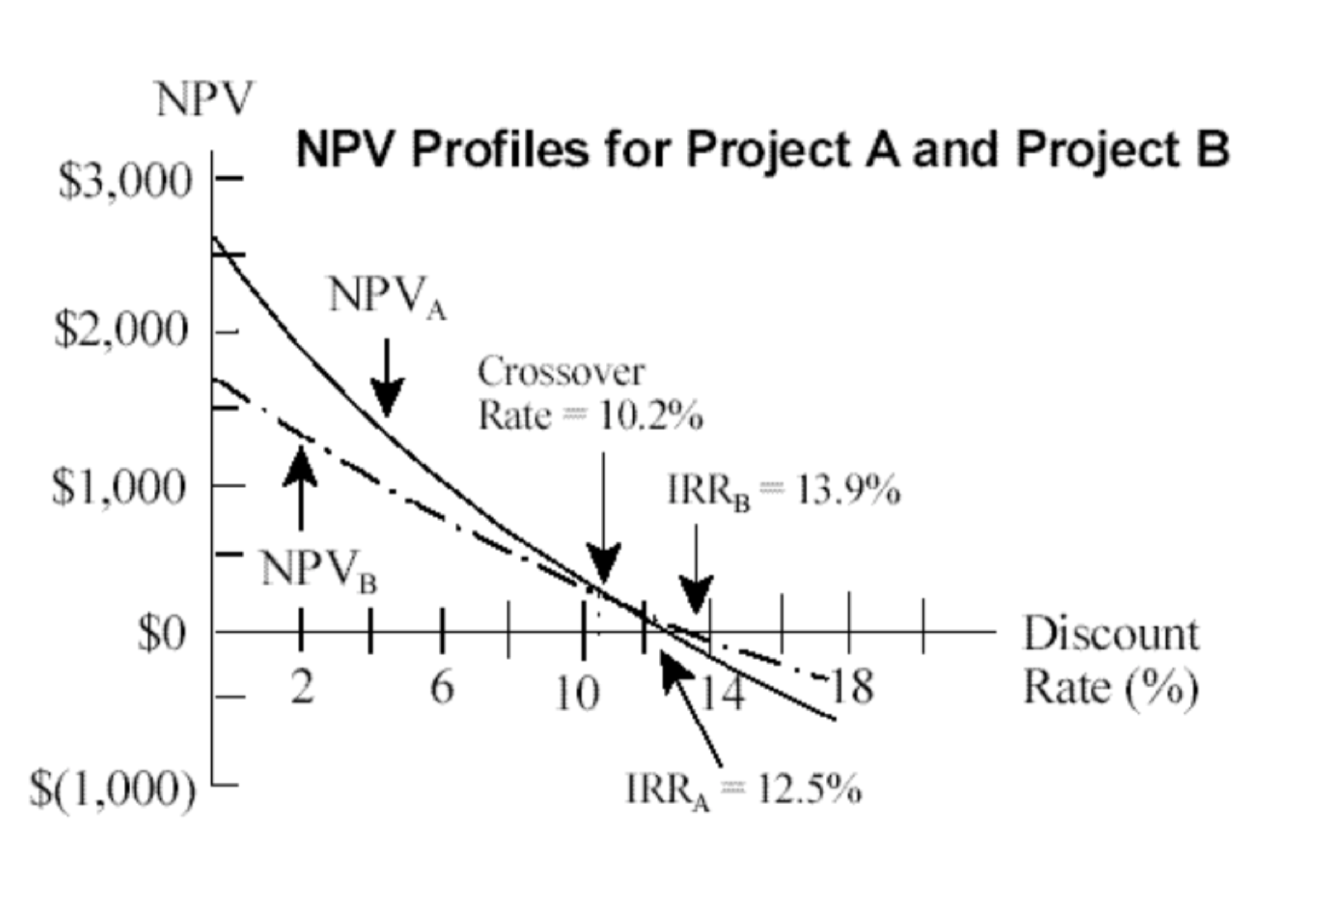
\includegraphics[width=0.5\linewidth]{images/van_vs_tir}
	\caption{Profili VAN per il progetto A e il progetto B}
	\label{fig:vanvstir}
\end{figure}

\vspace{1em}
Esaminando la \figurename ~\ref{fig:vanvstir} si nota che:
\begin{itemize}
	\item Con bassi tassi di sconto il progetto A mostra un VAN maggiore, mentre il progetto B ha un VAN
	maggiore a tassi più elevati. La spiegazione di tale andamento risiede nel fatto che, sebbene il
	progetto B generi flussi di cassa inferiori al progetto A, la distribuzione temporale di tali flussi è
	differente: B genera i flussi più consistenti nei primi anni, mentre per A avviene il contrario, per cui
	TIR B > TIR A
	\item La pendenza della curva è maggiore per il progetto A rispetto al progetto B, fatto che indica come il
	VAN del progetto A sia più sensibile ai cambiamenti nel tasso di sconto: variazioni nei tassi comportano variazioni maggiori nel VAN di A rispetto a B
\end{itemize}

Il punto in cui $VAN_A = VAN_B$, detto \emph{crossover rate}, si trova in corrispondenza di un tasso di sconto pari al
10.2\%. Tale valore può essere determinato prendendo le differenze tra i flussi di cassa dei due progetti e
calcolandone il relativo TIR.

\begin{tabular}{|c|r|r|r|}
	\hline
	\grayrow\multicolumn{4}{|c|}{Cash Flows} \\
	\hline
	\grayrow Anno & Progetto A & Progetto B & Differenza \\
	\hline
	0 & 5000 & 5000 & 0 \\
	\hline
	1 & 800 & 2400 & 1600 \\
	\hline
	2 & 900 & 1800 & 900 \\
	\hline
	3 & 1500 & 900 & 600 \\
	\hline
	4 & 1200 & 900 & 300 \\
	\hline
	5 & 3200 & 700 & 2500 \\
	\hline
\end{tabular}
\vspace{1em}

Se il tasso di sconto è < 10.2\% il VAN del progetto A è maggiore di quello del progetto B, mentre se il
tasso è > 10.2\% si verifica la situazione opposta.

\subsection{VAN vs PB}

I due indicatori considerano \emph{aspetti differenti} del progetto di investimento (redditività vs liquidità del
progetto): il PB period costituisce un \emph{valido complemento} agli indicatori precedentemente esposti.

\section{Schema riassuntivo}
\begin{itemize}
	\item \textbf{VAN}
	\begin{itemize}
		\item Accetto se VAN $> 0$
		\item Corrisponde al valore attuale dei flussi di cassa
		attesi, al netto dell’esborso iniziale per realizzare
il progetto
		\item Difficile scelta del tasso di attualizzazione
		\item Inadeguato per valutare investimenti con
rilevanza strategica
		\item Difficile stima dei flussi di cassa
	\end{itemize}
	\item \textbf{TIR}
	\begin{itemize}
		\item Accetto se TIR $> k$
		\item È il tasso di attualizzazione in corrispondenza del
quale risulta VAN $=0$
		\item Problemi se vi sono forti differenze tra tassi a breve/lungo nella struttura per scadenza dei tassi
di interesse
		\item Non sempre applicabile (flussi di cassa non
convenzionali)
	\end{itemize}
	\item \textbf{PI}
	\begin{itemize}
		\item Accetto se PI $> k$
		\item Misura l’entità dei benefici rispetto ai costi
		dell’investimento
		\item Essendo una variante del VAN presenta tutti i
		suoi limiti
		\item Effetto di scala
	\end{itemize}
	\item \textbf{PB Period}
	\begin{itemize}
		\item Accetto se PB Period $> k$
		\item Misura il momento nel quale i flussi in entrata
		attualizzati eguagliano il valore dei flussi in uscita
attualizzati
		\item Pone sullo stesso piano investimenti con tempo
		di recupero uguale, anche se comportano
esborsi iniziali diversi
	\end{itemize}
\end{itemize}